\documentclass[12pt]{article}
\usepackage{amsmath, amssymb, bm}
\usepackage{graphicx}
\usepackage{geometry}
\geometry{margin=1in}

\title{Holographic Entropic Spacetime (HES): A Toy Model for Emergent Curvature}
\author{Christopher Hanson-Graville \\ \small{Independent Researcher}}
\date{3 October 2025}


\begin{document}

\maketitle

\begin{abstract}
The nature of spacetime remains one of the deepest puzzles in theoretical physics. While General Relativity describes gravity as curvature in a geometric manifold, and Quantum Mechanics governs the probabilistic behavior of particles, a unified framework that explains how spacetime itself emerges from quantum principles remains elusive.

This paper introduces a toy model based on the Holographic Entropic Spacetime (HES) framework, where curvature arises from entropy gradients in a discrete lattice of microstates. The model simulates how local entropic interactions and global feedback dynamics can generate stable geometric structure without invoking mass or classical fields. We present a reproducible benchmark notebook that visualizes this process, offering a hands-on demonstration of how information structure alone can give rise to curvature. The results support the hypothesis that spacetime may be a macroscopic manifestation of underlying entropic dynamics—and open new avenues for exploring emergent gravity from first principles.
\end{abstract}

\section{Introduction}

The nature of spacetime remains one of the deepest puzzles in theoretical physics. While General Relativity describes gravity as curvature in a geometric manifold, and Quantum Mechanics governs the probabilistic behavior of particles, a unified framework that explains how spacetime itself emerges from quantum principles remains elusive.

Recent advances in quantum information theory suggest that entanglement may play a foundational role in the emergence of spacetime geometry. The idea that “geometry is entanglement” has gained traction—but concrete, reproducible models remain rare.

This paper introduces a toy model based on the Holographic Entropic Spacetime (HES) framework, where curvature arises from entropy gradients in a discrete lattice of microstates. The model simulates how local entropic interactions and global feedback dynamics can generate stable geometric structure without invoking mass or classical fields.

We present a reproducible benchmark notebook that visualizes this process, offering a hands-on demonstration of how information structure alone can give rise to curvature. The results support the hypothesis that spacetime may be a macroscopic manifestation of underlying entropic dynamics—and open new avenues for exploring emergent gravity from first principles.

\section{Theoretical Framework}

The Holographic Entropic Spacetime (HES) model proposes that spacetime curvature can emerge from entropy gradients across a discrete lattice of quantum microstates. This framework is inspired by the idea that information structure—not mass or classical fields—may be the true substrate of geometry.

\subsection{Microstate Lattice and Entropy Field}

We begin with a two-dimensional lattice `\( S(x, y) \)`, where each site represents a quantum microstate. The entropy at each site is initialized randomly within a bounded range, and evolves over time according to local interactions and global feedback.

The entropy field is visualized as a heatmap, with color intensity representing the value of `\( S(x, y) \)`. This field serves as the foundation for curvature extraction.

\subsection{Informational Action and Feedback Loop}

To simulate global coherence, we define an Informational Action `\( \mathcal{A}(t) \)`, which aggregates entropic flows across the lattice. Arrows between neighboring sites represent directional entropic gradients, and a feedback loop overlays the system to enforce temporal consistency.

This feedback mechanism is schematic, but conceptually analogous to an action principle in classical physics—minimizing `\( \mathcal{A}(t) \)` leads to emergent structure.

\subsection{Curvature Extraction via Laplacian}

Curvature is derived from the entropy field using a discrete Laplacian operator:

\begin{equation}
C(x, y) = \nabla^2 S(x, y)
\end{equation}

This yields a curvature map `\( C(x, y) \)`, which is visualized as a second heatmap. Positive curvature corresponds to regions of high entropy concentration, while negative curvature reflects entropic depletion.

\subsection{Update Rule: Metropolis–Hastings}

The lattice evolves via a Metropolis–Hastings algorithm. At each timestep, a candidate microstate flip is proposed and accepted probabilistically based on its impact on the global entropy configuration.

This rule ensures that the system explores its configuration space while favoring transitions that reduce informational tension. Over time, the lattice stabilizes into a geometry shaped by entropic dynamics.

\begin{figure}[ht]
    \centering
    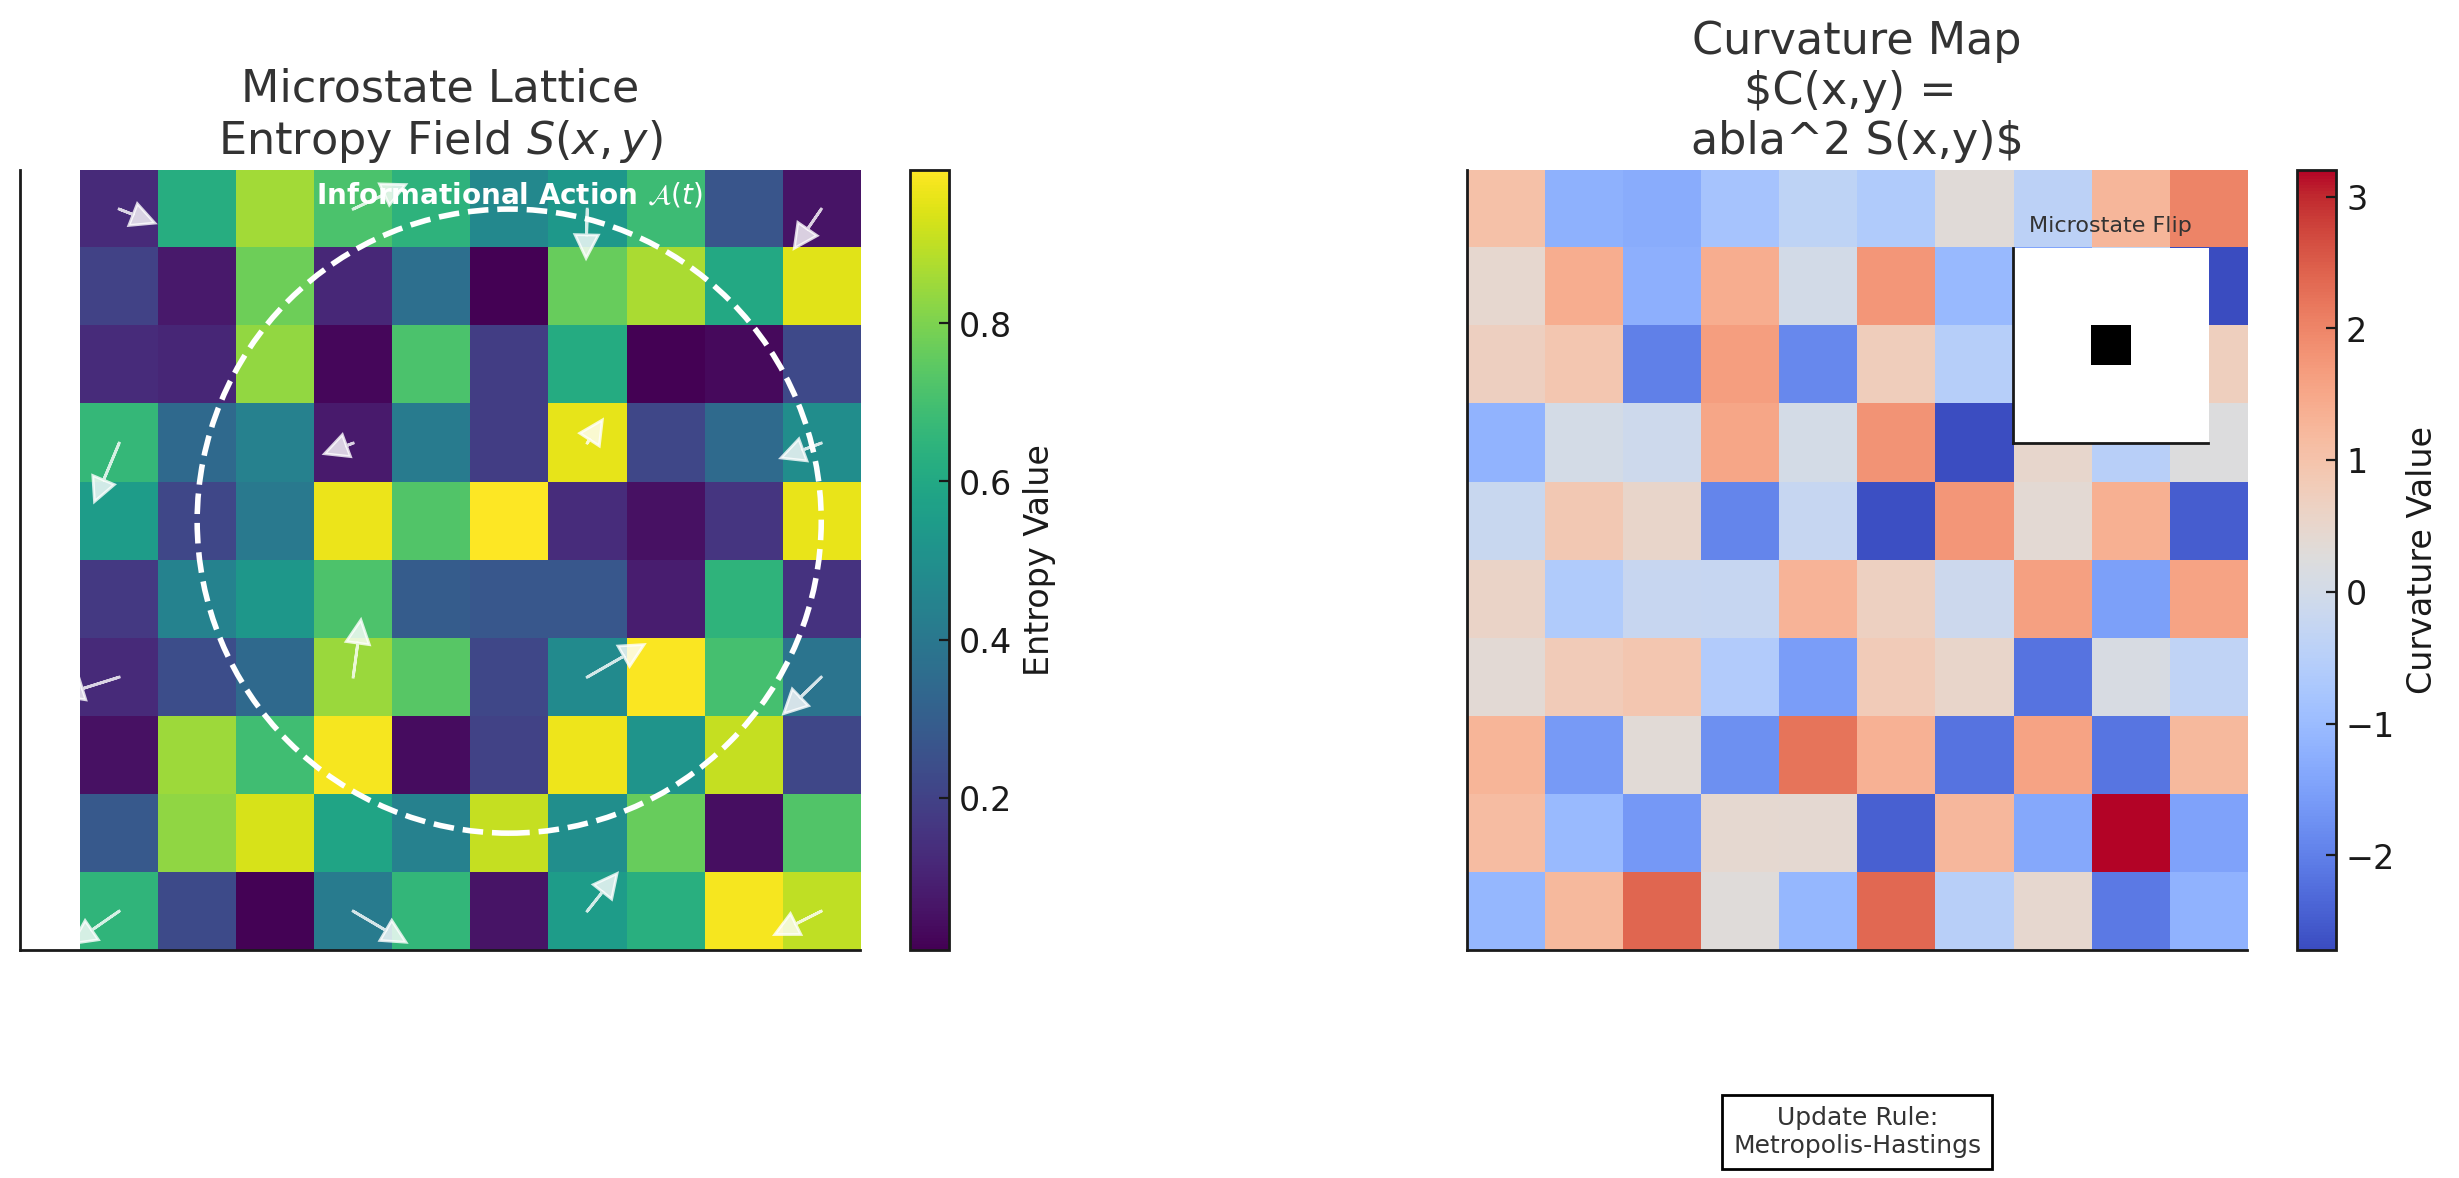
\includegraphics[width=0.9\textwidth]{Figures/Figure_5.png}
    \caption{
        Schematic illustration of the Holographic Entropic Spacetime (HES) framework.  
        \textbf{Left:} A 2D microstate lattice with entropy field `\( S(x, y) \)`, color-coded from low (purple) to high (yellow) entropy. Arrows represent schematic entropic flows, and a dashed loop labeled `\( \mathcal{A}(t) \)` indicates global informational feedback.  
        \textbf{Right:} The derived curvature map `\( C(x, y) = \nabla^2 S(x, y) \)`, color-coded from negative (blue) to positive (red) curvature. An inset highlights a microstate flip governed by the Metropolis–Hastings update rule.
    }
    \label{fig:HES_schematic}
\end{figure}



